% ==============================================================================
% EXPERIMENTOS
% ==============================================================================
% Instrucciones de la plantilla:
% - Detallar de manera clara y estructurada las pruebas realizadas.
% - Incluir tanto los resultados exitosos como los fallidos.
% - Detallar las variaciones exploradas en cada actividad.
% - Describir los experimentos base: objetivo, metodología empleada y resultados obtenidos, respaldados con imágenes, gráficos o datos numéricos.
% ==============================================================================

\section{Experimentos}

En esta sección se presentan las pruebas experimentales desarrolladas para validar el comportamiento del sistema gráfico bajo distintas configuraciones y parámetros.

\subsection{Experimento 1: [Título o variación probada]}
\subsubsection{Objetivo del experimento}
Evaluar el comportamiento del renderizado al variar los parámetros de...

\subsubsection{Pruebas exitosas}
% Describir casos en los que la prueba funcionó como se esperaba:
Se observó que al configurar... la salida gráfica generó la geometría esperada con una tasa de cuadros estable.

\subsubsection{Pruebas fallidas y análisis de errores}
% Describir fallos encontrados durante el desarrollo, errores de compilación/enlace/shaders:
Durante la primera ejecución ocurrió un fallo debido a una discrepancia en el formato de los atributos del vértice (layout del shader), provocando una pantalla en negro (\textit{black screen}). Dicho error se corrigió ajustando el paso (\textit{stride}) en \texttt{glVertexAttribPointer}.

%\begin{figure}[H]
%    \centering
%    \includegraphics[width=0.7\textwidth]{Imagenes/experimento_error.png}
%    \caption{Captura del comportamiento erróneo observado antes de la corrección.}
%    \label{fig:error_exp1}
%\end{figure}

\subsection{Experimento 2: [Título o variación probada]}
% Detallar los experimentos para la siguiente actividad o variante explorada.
\textit{Describir aquí el segundo experimento realizado, sus variaciones y contrastes...}

\subsection{Experimentos de la Actividad 3: segundo personaje de Mixamo}

\subsubsection{Objetivo del experimento}
La variación de esta actividad fue sustituir el personaje de ejemplo del laboratorio por uno descargado por nosotros (Exo Gray) y comprobar qué tanto hay que adaptar un modelo de Mixamo para que lo anime el mismo cargador. El personaje de ejemplo se conservó en el programa para comparar los dos directamente con la tecla \texttt{G}.

\subsubsection{Pruebas fallidas y análisis de errores}
\textbf{Piernas colapsadas.} La primera versión ya tenía una sola malla y un solo material, y aun así, al ejecutar el programa, el torso, los brazos y la cabeza se veían y se animaban bien, pero las dos piernas salían convertidas en picos que se estiraban desde la rodilla hasta un punto en el piso (Figura \ref{fig:piernas_colapsadas}). Lo primero que descartamos fueron los pesos: revisamos en Blender las influencias de cada vértice y ninguno tenía más de cuatro huesos, y en todos los pesos sumaban exactamente 1.

\begin{figure}[H]
    \centering
    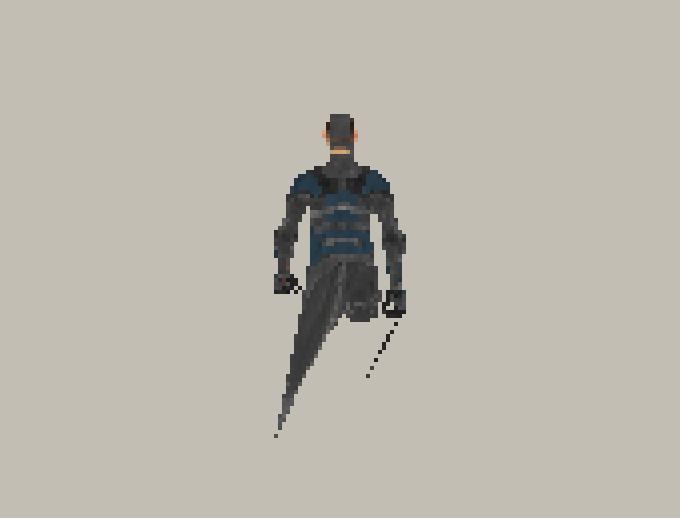
\includegraphics[width=0.45\textwidth]{Imagenes/E3/03_opengl_piernas_colapsadas.png}
    \caption{Primera carga de Exo Gray en OpenGL (acercamiento): la parte superior del cuerpo se anima correctamente, pero los vértices de las piernas se colapsan hacia el origen del modelo.}
    \label{fig:piernas_colapsadas}
\end{figure}

La pista estuvo en la forma del error: un vértice multiplicado por una matriz nula termina en el origen del modelo, que en un personaje de Mixamo está justo entre los pies. Al listar la armadura por índice encontramos que el exportador FBX de Blender escribe un \textit{cluster} por \emph{cada} hueso de la armadura, tenga pesos o no; con 112 huesos, los de las piernas (\texttt{LeftUpLeg} a \texttt{RightToeBase}) quedaban con los índices 102 a 110, fuera del arreglo \texttt{gBones[100]} del \textit{shader}. La parte superior funcionaba simplemente porque sus huesos aparecen antes en el árbol. La corrección fue borrar los 18 huesos sin pesos, todos hojas, con lo que la armadura bajó a 94 huesos y las piernas a índices menores que 100.

\textbf{Animación congelada.} En la misma prueba la consola reportó \texttt{Animation total frames: 249} para Exo Gray, cuando el clip de Mixamo tiene 32 cuadros. El exportador hornea la animación sobre el rango de la escena de Blender, que por omisión va de 1 a 250, así que el personaje daba un ciclo de caminata y se quedaba quieto en la última pose durante unos siete segundos antes de reiniciar. Se corrigió ajustando el rango de la escena al de la acción antes de exportar; después de eso la consola reporta 31 cuadros para los dos personajes.

\subsubsection{Pruebas exitosas}
Con las dos correcciones, Exo Gray se carga como una sola malla de 16\,738 vértices, con su textura completa, y camina sin deformaciones. Como comparación, el personaje de ejemplo tiene 2\,456 vértices y 68 huesos. La diferencia de tamaño sí se nota en un aspecto: \texttt{AnimatedModel} asigna los pesos recorriendo, para cada vértice, todos los pesos de todos los huesos, por lo que el tiempo de carga crece con el producto de ambos, y con Exo Gray el programa tarda alrededor de medio minuto en mostrar la escena.

\subsection{Experimentos de la Actividad 4: zona ampliada con casas, calles y banquetas}

\subsubsection{Objetivo del experimento}
La variación de esta actividad fue generar los alrededores a partir de las medidas de la ciudad en lugar de colocarlos a mano, para verificar que el mismo procedimiento se adapta a una ciudad de otro tamaño sin rehacer el modelado.

\subsubsection{Pruebas exitosas}
El guion se escribió primero sobre una versión preliminar de la ciudad que ocupaba $x \in [-2.2,\ 72]$ y $y \in [-20,\ 4]$, y con ella dejaba 7 casas por fila. Al cambiar al modelo definitivo de la Actividad 1, que es más angosto en $X$ y bastante más profundo en $Y$, no fue necesario tocar ninguna medida: el guion recalculó las manzanas a $79 \times 51$ unidades, bajó el número de casas a 6 por fila, ajustó la separación del segundo \textit{Array} de las casas a 89 unidades y la de las líneas de las avenidas a 63 unidades. Las casas, con sus puertas y ventanas, no cambiaron en absoluto, porque su modelado no depende del tamaño de la ciudad.

\subsubsection{Pruebas fallidas y análisis de errores}
En la primera ejecución en OpenGL la mayor parte de la ventana quedó cubierta por una superficie gris clara y el personaje no aparecía (Figura \ref{fig:camara_techo}). La cámara se había colocado a 6 unidades de altura y a $z = 50$, que en la ciudad ampliada cae justo sobre la fila de casas de enfrente; como el techo de las casas llega exactamente a 6 unidades, la cámara quedó dentro de uno de ellos. La corrección fue subirla a 10 unidades de altura e inclinarla $20^\circ$ hacia abajo, de modo que queda por encima de los techos y sigue viendo al personaje sobre la avenida.

\begin{figure}[H]
    \centering
    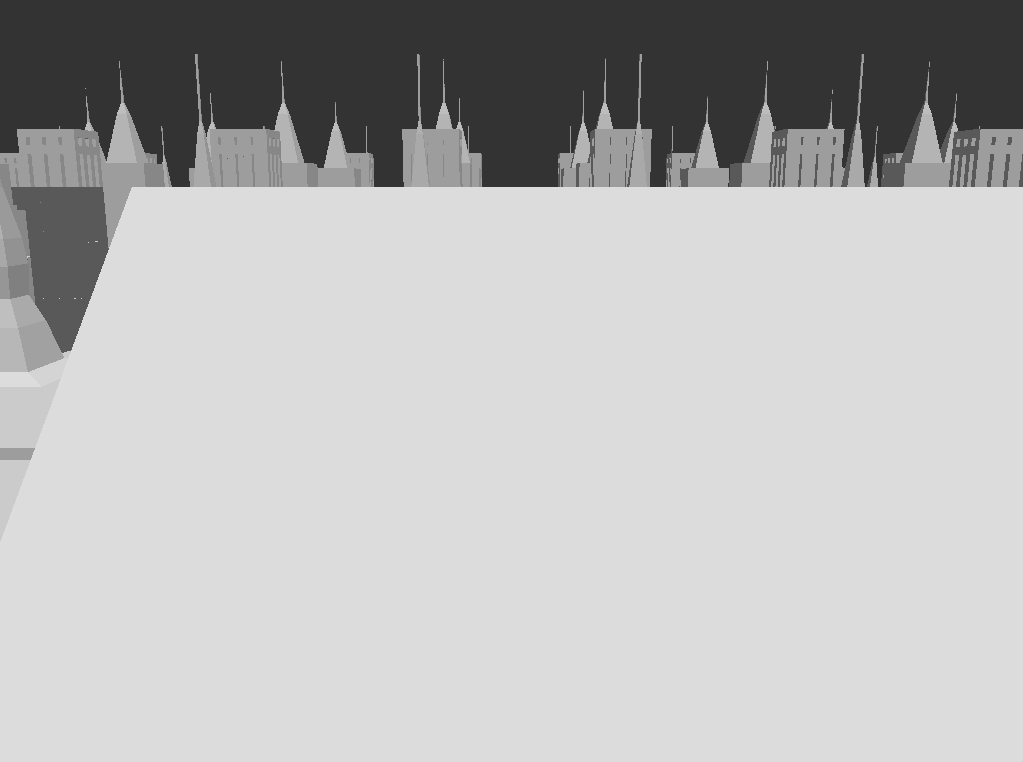
\includegraphics[width=0.6\textwidth]{Imagenes/E4/12_opengl_camara_dentro_techo.png}
    \caption{Primera ejecución de la zona ampliada en OpenGL: la cámara quedó dentro del techo de una casa de la fila de enfrente y el techo cubre casi toda la vista.}
    \label{fig:camara_techo}
\end{figure}